\documentclass[11pt]{article}

\setlength{\oddsidemargin}{0.1in}
\setlength{\textwidth}{6.5in}
\setlength{\topmargin}{-0.5in}
\setlength{\textheight}{9in}
\renewcommand{\baselinestretch}{1.3} 

\usepackage{fancyhdr}
%%\usepackage{fullpage}
%%\usepackage{subfigure}
\usepackage{latexsym}
\usepackage{wrapfig}
\usepackage{graphicx}
\usepackage{amsmath, amsthm, amssymb}
\usepackage{natbib}
\usepackage{algorithm}
\usepackage{algorithmic}
\numberwithin{algorithm}{section}
%%\usepackage{amsfonts}
%\usepackage{nopageno}

%%\usepackage{graphicx}        % standard LaTeX graphics tool
                             % when including figure files
%%\usepackage{multicol}        % used for the two-column index
%%\usepackage[bottom]{footmisc}% places footnotes at page bottom


%% my additional packages 
%%\usepackage{lscape}
%%\usepackage{fancybox}
%%\usepackage{amsfonts,amssymb,amsfonts,amsmath}
%%\usepackage{threeparttable}




%\newcommand{\draftnote}[1]{\marginpar{\tiny\raggedright\textsf{\hspace{0pt}{\bf Comments}:#1}}}
%\newcommand{\draftnote}[1]{}

%%\DeclareMathOperator*{\argmax}{arg\,max}

\newcommand{\cprob}[2]{\ensuremath{\text{Pr}\left(#1 \,|\,#2\right)}}  
\newcommand{\prob}[1]{\ensuremath{\text{Pr}\left(#1 \right)}}
\newcommand{\cexpect}[4]{\ensuremath{\text{E}\left#3 #1 \,|\,#2\right#4}}  
\newcommand{\expect}[3]{\ensuremath{\text{E}\left#2 #1 \right#3}}

\newcommand{\fder}[1]{\frac{d}{d #1}}
\newcommand{\hder}[2]{\frac{d^{#2}}{d {#1}^{#2}}}
\newcommand{\fpart}[1]{\frac{\partial}{\partial #1}}
\newcommand{\hpart}[2]{\frac{\partial^{#2}}{\partial {#1}^{#2}}}
\newcommand{\iid}{\ensuremath{\overset{\text{iid}}{\sim}}}
\newcommand{\indfun}[1]{\ensuremath{1_{\{#1\}}}}
\newcommand{\asarrow}{\ensuremath{\overset{\text{a.s.}}{\rightarrow}}}
\newcommand{\parrow}{\ensuremath{\overset{\text{P}}{\rightarrow}}}
\newcommand{\darrow}{\ensuremath{\overset{\text{D}}{\rightarrow}}}
\newcommand{\mydef}{\ensuremath{\overset{\text{def}}{=}}}

\DeclareMathOperator*{\argmax}{arg\,max}
\DeclareMathOperator*{\argmin}{arg\,min}

\newtheorem*{theorem}{Theorem}
\newtheorem*{prop}{Proposition}
\newtheorem*{corollary}{Corollary}
\newtheorem*{lemma}{Lemma}

\theoremstyle{remark}
\newtheorem*{mynote}{Note}

\theoremstyle{definition}
\newtheorem*{define}{Definition}

\newenvironment{example}[1]{\begin{trivlist}
\item[\hskip \labelsep {\bfseries Example}: \underline{#1}]\ \\}{\end{trivlist}}

\newenvironment{Proof}{\begin{trivlist}
\item[\hskip \labelsep \textit{Proof}:]}{\end{trivlist}}

\newenvironment{exercise}{\begin{trivlist}
\item[\hskip \labelsep \textit{Exercise}:]}{\end{trivlist}}

\newcommand{\todo}[1]{\begin{center}To do: {\bf #1}\end{center}}

%% group numberging of equations and figures by section

\numberwithin{equation}{section}
\numberwithin{figure}{section}

\bibliographystyle{plainnat}


\pagestyle{fancy}
\renewcommand{\headrulewidth}{0.8pt}
\lhead{\bf \large SISMID, Module 8 Practicals}
\rhead{\bf Summer 2017}
\chead{} 
\lfoot{} 
\rfoot{} 
\cfoot{}

\begin{document}

\setkeys{Gin}{width=1.0\textwidth}


\begin{center}
  \textbf{\Large Practical: Monte Carlo and Markov chain theory}\\
  {\large Instructors: Kari Auranen, Elizabeth Halloran and Vladimir Minin}\\
  {\large July 17 -- July 19, 2017}
\end{center}


\section*{Estimating the tail of the standard normal distribution}
  Let $Z \sim \mathcal{N}(0,1)$. We would like to estimate the tail probability 
  $\text{Pr}(Z > c)$, where $c$ is large (e.g., $c = 4.5$).  
  \par
  \textit{Naive Monte Carlo}: simulate $Z_1,\dots,Z_n {\buildrel \text{iid} \over \sim} \mathcal{N}(0,1)$.
  Then 
  \begin{equation*}
    \hat{\mu} = \frac{1}{n} \sum_{i=1}^n 1_{\{Z_i>c\}} \approx 
   \text{E}\left(1_{\{Z>c\}}\right) = \text{Pr}(Z>c). 
  \end{equation*}
  This estimator will most likely give you 0 even for $n = 10,000$.  
  The problem is the large variance of the integrand:
  \begin{equation*}
    \text{Var}(\hat{\mu}) = \frac{1}{n}\text{Var}(\indfun{Z_1 > c}) 
    = \frac{1}{n}\text{Pr}(Z_1 > c)[1 - \text{Pr}(Z_1 > c)] = \mathbf{3.4\times10^{-10}} \text{ for } n=10,000 
    \text{ and } c=4.5. 
  \end{equation*}
  This variance is huge, because the quantity of interest is $\text{Pr}(Z_1 > c) = 3.39\times 10^{-6}$ and the standard
  deviation of our estimator is $1.84\times10^{-5}$.
  \par
  \textit{Importance sampling}: Simulate $Y_1,...,Y_n {\buildrel \text{iid} \over \sim} \text{Exp}(c, 1)$ 
  from a shifted exponential with density
  \begin{equation*}
    g(y) = e^{-(y-c)}1_{\{y > c\}}.
  \end{equation*}
  Generating such random variables is very easy: just simulate a regular exponential $\text{Exp}(1)$ and
  add $c$ to the simulated value. Then the importance sampling estimator becomes
  \begin{equation*}
    \tilde{\mu} = \frac{1}{n} \sum_{i=1}^n \frac{\phi(Y_i)}{g(Y_i)} \indfun{Y_i > c},
  \end{equation*}
  where $\phi(x)$ is the standard normal density. The variance of this estimator amounts to 
  \begin{equation*}
    \begin{split}
      \text{Var}(\tilde{\mu}) &= \frac{1}{n} \text{Var}\left[ 
        \frac{\phi(Y)}{g(Y)}1_{\{Y > c\}}\right] = 
      \frac{1}{n}\left\{\text{E}_g\left[\frac{\phi^2(Y)}{g^2(Y)}1_{\{Y > c\}}\right] 
        - \left[\text{E}_g\left(\frac{\phi(Y)}{g(Y)}1_{\{Y > c\}}\right)\right]^2\right\} \\ 
      &=\frac{1}{n}\left[\int_c^\infty \frac{\phi^2(y)}{g(y)}dy - \text{Pr}(Z > c)^2\right] 
      = \mathbf{1.9474\times 10^{-15}} \text{ for } n=10,000 \text{ and } c=4.5.
    \end{split}
  \end{equation*}
  This means that we reduced Monte Carlo variance roughly by a factor of $10^5$ using importance 
  sampling.


\subsection*{Your task}
Implement naive and importance sampling Monte Carlo estimates of $\text{Pr}(Z>4.5)$, where
$Z \sim \mathcal{N}(0,1)$. Download `import\_sampl\_reduced.R' from 
the course web page. The code has a couple of things to get you started.

\section*{Ehrenfest model of diffusion}
Imagine a two dimensional rectangular box with a divider in the middle. The box contains $N$ balls
(gas molecules)  distributed somehow between the two halves. The divider has a small gap, through which 
balls can go through one at a time. We assume that at each time step we select a ball uniformly at 
random and force it go through the gap to the opposite side of the divider. Letting $X_n$ denote
the total number of balls in the left half of the box, our Markov process is described by the 
following transition probabilities.

\begin{minipage}[c]{0.5\textwidth}
  \[
  p_{ij} =
  \begin{cases}
    \frac{i}{N}. &\text{ for } j=i-1,\\\
    1-\frac{i}{N}, &\text{ for } j=i+1,\\
    0, \text{ otherwise}.
  \end{cases}
  \]
\end{minipage}
\begin{minipage}[r]{0.45\textwidth}
  \vspace{0.2cm}
  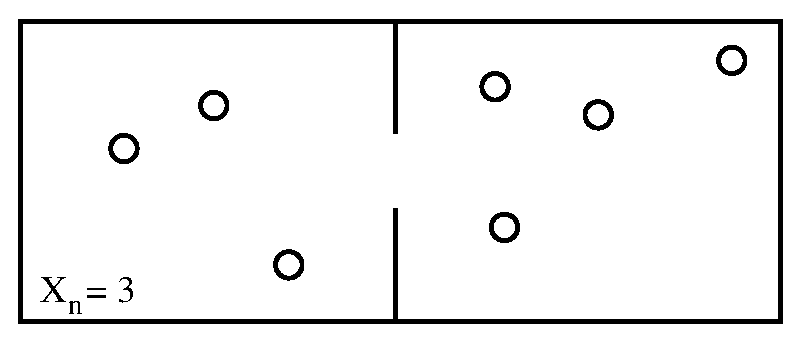
\includegraphics[width=0.9\textwidth]{ehrenfest}
  \vspace{0.3cm}
\end{minipage}

If we want to derive a stationary distribution of the system, we can solve the global balance equations
$\boldsymbol{\pi}^T \mathbf{P} = \boldsymbol{\pi}^{T}$. Alternatively, we may ``guess'' that at
equilibrium $X_n \sim \text{bin}(\frac{1}{2}, N)$ and verify this candidate stationary distribution
via detailed balance. Notice we do not know whether the Ehrenfest chain is reversible, but we'll go
ahead with the detailed balance check anyway. First, notice that entries of our candidate vector are
\begin{equation*}
  \pi_i = {N \choose i} \left(\frac{1}{2}\right)^i\left(1-\frac{1}{2}\right)^{N-i} = 
  {N \choose i} \frac{1}{2^N}
\end{equation*}
Since $X_n$ can only increase or decrease by one at each time step, we need to check detailed balance 
only for $i$ and $j = i + 1$.  
\[
\begin{split}
  &\pi_i p_{i,i+1} = \frac{1}{2^N}{N \choose i} \frac{N - i}{N} =
  \frac{1}{2^N} \frac{N!}{i!(N-i)!} \frac{N - i}{N} =
  \frac{1}{2^N} \frac{N!}{(i+1)!(N-i-1)!} \frac{i+1}{N}\\
  &= {N \choose i+1} \frac{1}{2^N} \frac{i+1}{N} = \pi_{i+1} p_{i+1,i},
\end{split}
\]
confirming our guess.
\par
Now, consider the Ehrenfest model with $N=100$ gas molecules. 
From our derivations we know that 
  the stationary distribution of the chain is $\text{Bin}(\frac{1}{2},N)$. The chain is irreducible
  and positive recurrent (why?). The stationary variance can be computed analytically as 
  $N\times\frac{1}{2}\times\frac{1}{2}$. 

\subsection*{Your task}
Use ergodic theorem to approximate the stationary variance and compare your estimate with the analytical result.
Don't panic! You will not have to write everything from scratch. Download `ehrenfest\_diff\_reduced.R' file from the course
web page. Follow comments in this R script to fill gaps in the code. 




\end{document}

